% compile with XeLaTeX
% this template was created by salim bou 
\documentclass[dvipsnames,mathserif]{beamer}
\usepackage{setspace, float}
\setstretch{1.2}
\usepackage{tikz}
\usepackage{subcaption}

\usepackage{amsmath, amssymb, amsthm, nicematrix}

\usepackage{polyglossia}
\setdefaultlanguage[numerals=maghrib,locale=algeria]{arabic} % locale=mashriq, libya, algeria, tunisia, morocco, or mauritania  for names of months in \date 
\setotherlanguage{english}
\newfontfamily\arabicfont[Script=Arabic]{Amiri}
\newfontfamily\arabicfontsf[Script=Arabic]{Amiri}
\newfontfamily{\timesfont}{Times New Roman}

\newcommand{\ar}{\textarabic}
\newcommand{\en}{\textenglish}

\usepackage[T1]{fontenc}
\usepackage{times}

\usepackage[lite, zswash]{mtpro2}

\DeclareMathSymbol{0}{\mathalpha}{operators}{`0}
\DeclareMathSymbol{1}{\mathalpha}{operators}{`1}
\DeclareMathSymbol{2}{\mathalpha}{operators}{`2}
\DeclareMathSymbol{3}{\mathalpha}{operators}{`3}
\DeclareMathSymbol{4}{\mathalpha}{operators}{`4}
\DeclareMathSymbol{5}{\mathalpha}{operators}{`5}
\DeclareMathSymbol{6}{\mathalpha}{operators}{`6}
\DeclareMathSymbol{7}{\mathalpha}{operators}{`7}
\DeclareMathSymbol{8}{\mathalpha}{operators}{`8}
\DeclareMathSymbol{9}{\mathalpha}{operators}{`9}

\usetheme{Warsaw}
%\usecolortheme{crane}

% for RTL liste
\makeatletter
\newcommand{\RTListe}{\raggedleft\rightskip\leftm}
\newcommand{\leftm}{\@totalleftmargin}
\makeatother



% RTL frame title
\setbeamertemplate{frametitle}
{\vspace*{-1mm}
	\nointerlineskip
	\begin{beamercolorbox}[sep=0.3cm,ht=2.2em,wd=\paperwidth]{frametitle}
		\vbox{}\vskip-2ex%
		\strut\hskip1ex\insertframetitle\strut
		\vskip-0.8ex%
	\end{beamercolorbox}
}


% align subsection in toc
\makeatletter
\setbeamertemplate{subsection in toc}
{\leavevmode\rightskip=5ex%
	\llap{\raise0.1ex\beamer@usesphere{subsection number projected}{bigsphere}\kern1ex}%
	\inserttocsubsection\par%
}
\makeatother

% RTL triangle for itemize
\setbeamertemplate{itemize item}{\scriptsize\raise1.25pt\hbox{\donotcoloroutermaths$\blacktriangleleft$}} 

%\setbeamertemplate{itemize item}{\rule{4pt}{4pt}}

\defbeamertemplate{enumerate item}{square2}
{\LR{
		%
		\hbox{%
			\usebeamerfont*{item projected}%
			\usebeamercolor[bg]{item projected}%
			\vrule width2.25ex height1.85ex depth.4ex%
			\hskip-2.25ex%
			\hbox to2.25ex{%
				\hfil%
				{\color{fg}\insertenumlabel}%
				\hfil}%
		}%
}}

\setbeamertemplate{enumerate item}[square2]

\setbeamertemplate{navigation symbols}{}





\author{\textbf{الطالبة : زهراء كريم}}
\title{\textbf{من تطبيقات الجبر الخطي}}
\date{\textbf{اشراف : م. تهاني عبدالمجيد}}
\begin{document}
	\abovedisplayskip=0pt
	\belowdisplayskip=0pt
	\maketitle
	\timesfont
	
	\begin{frame}
		\begin{figure}
			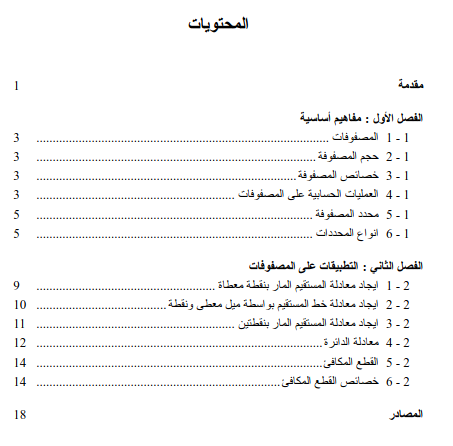
\includegraphics[scale=0.6]{contents.png}
		\end{figure}
	\end{frame}
	
	\begin{frame}{مقدمة}
		\noindent
		المصفوفات هي إحدى أهم البنى الرياضية التي تُستخدم على نطاق واسع في الرياضيات والهندسة والعلوم التطبيقية. تتكون المصفوفة من مجموعة من الأعداد أو الرموز مرتبة في صفوف وأعمدة داخل جدول مستطيل الشكل، مما يسهل التعامل مع البيانات وتمثيل الأنظمة المعقدة بطريقة منظمة وفعالة.\\
		\noindent
		تلعب المصفوفات دورًا حيويًا في العديد من المجالات، مثل الجبر الخطي، الإحصاء، الفيزياء، والهندسة. ومن أبرز تطبيقاتها:
		\begin{itemize}
			\item \textbf{تمثيل وحل الأنظمة الخطية:} حيث تُستخدم لحل مجموعة من المعادلات الخطية بطريقة مبسطة باستخدام العمليات المصفوفية مثل ضرب المصفوفات وعكسها.
			\item \textbf{تحليل البيانات والذكاء الاصطناعي:} إذ تُستخدم في معالجة الصور، التعلم العميق، وتحليل البيانات الكبيرة.
			\item \textbf{فيزياء الكم والرسومات الحاسوبية:} حيث تُستخدم في تدوير الأجسام وتحويل الإحداثيات في الفضاء ثلاثي الأبعاد.
		\end{itemize}
	\end{frame}
	
	\begin{frame}
		\begin{center}
			\Huge
			\textbf{الفصل الاول}\\
			\textbf{مفاهيم اساسية}
		\end{center}
	\end{frame}
	
	\begin{frame}
		\begin{exampleblock}{المصفوفات}
			يمكن تعريف المصفوفات بأنها ترتيب معين للاعداد على شكل اعمدة وصفوف . تكتب المصفوفات عادة على شكل صندوق مربع او مستطيل الشكل ويسمى الخط العمودي داخل المصفوفة بالعمود اما الخط الافقي فيسمى صفاً ويمكن التعبير عن حجم المصفوفة من خلال عدد الصفوف والاعمدة التي تحتويها كما يلي
		\end{exampleblock}
		
		\begin{exampleblock}{حجم المصفوفة}
			هو عدد الصفوف وعدد الاعمدة فمثلاً اذا كان عدد الصفوف في مصفوفة ما هو 2 وعدد الاعمدة هو 3 فإنه يتم التعبير عن حجمها بـــ $2\times3$ وهكذا. وتعرف المصفوفات والاعمدة بأبعاد المصفوفة.
		\end{exampleblock}
	\end{frame}
	
	\begin{frame}{العمليات على المصفوفات}
		\begin{exampleblock}{1 - جمع وطرح المصفوفات}
			يجب عند جمع او طرح المصفوفات ان تكون متساوية في الحجم اي يجب لعدد الصفوف والاعمدة ان يكون متساوياُ في كلا المصفوفتين.\\
			\noindent
			\textbf{مثال توضيحي:} اذا كان عدد الصفوف في مصفوفة ما 3 صفوف و 5 اعمدة فإنه يمكن جمعها مع مصفوفة اخرى اذا كان عدد صفوفها 3 صفوف وعدد اعمدتها 5. وفي المقابل لا يمكن مثلاً جمعها الى مصفوفة اخرى عدد الصفوف فيها 3 وعدد اعمدتها 4.\\
			ويتم الجمع عن طريق جمع كل عنصر متطابقين في الموقع بين المصفوفتين وكذلك الامر في عملية الطرح.
		\end{exampleblock}
	\end{frame}
	
	\begin{frame}{العمليات على المصفوفات}
		\begin{exampleblock}{2 - ضرب المصفوفات}
			يمكن ضرب مصفوفتين ببعضهما فقط اذا كان عدد الاعمدة في المصفوفة الاولى مساوياً لعدد الصغوف في المصفوفة الثانية ليكون حجم المصفوفة الناتجة هو عدد صفوف المصفوفة الاولى × عدد اعمدة المصفوفة الثانية
		\end{exampleblock}
		
		\begin{exampleblock}{مثال}
			\[
			A = 
			\begin{bmatrix}
				2 & 3 & 1\\
				2 & -7 &4
			\end{bmatrix}_{2\times 3}
			, B =
			\begin{bmatrix}
				3 &4& 5\\
				1 &1 &4\\
				2 &1& 4 
			\end{bmatrix}_{3\times 3}
			\]
			حجم المصفوفة الناتجة 
			\[
			[A]_{2\times \textcolor{red}{3}}\cdot [B]_{\textcolor{red}{3}\times 3} \Rightarrow [AB]_{2\times 3}
			\]
			\[
			AB = 
			\begin{bmatrix}
				11& 12& 26\\
				7 &5& -2 
			\end{bmatrix}_{2\times 3}
			\]
		\end{exampleblock}
	\end{frame}
	
	\begin{frame}
		\begin{exampleblock}{محدد المصفوفة}
			المحدد هو دالة رياضية تعتمد على بعد المصفوفة $n$ ويربط بقيمة قياسية (scalar) هي $\det A$ بكل مصفوفة مربعة $n\times n$ والمعنى الهندسي الاساسي للمحدد هو أنه بمثابة عامل المقياس للحجم عندما تعد المصفوفة $A$ تحويلا خطيا ويرمز عادة للمحدد لمصفوفة ما بالرمز $|A|$ . ولا يمكن حساب المحدد الا للمصفوفة المربعة
		\end{exampleblock}
		
		\begin{exampleblock}{تعريف}
			 لتكن $A$ مصفوفة مربعة من الدرجة $n$ اي ان $A=[a_{ij}]_n$ وتساوي
			\[
			A =
			\begin{bmatrix}
				a_{11} & a_{12} & \cdots & a_{1n}\\
				a_{21} & a_{22} & \cdots & a_{2n}\\
				\vdots & \vdots & \ddots & \vdots\\
				a_{n1} & a_{n2} & \cdots & a_{nn}\\
			\end{bmatrix}
			\] 
			ندعوا الرمز $|A|$ او $\det A$ بمحدد المصفوفة من الرتبة $n$ ونكتب
			\[
			|A| = |A|_n = |a_{ij}|_{n} = \det A
			\]
		\end{exampleblock}
	\end{frame}
	
	\begin{frame}{انواع المحددات}
		\begin{exampleblock}{المحدد من الرتبة الاولى}
			\[
			A = [a_{11}] \Rightarrow |A|_1 = |a_{11}|
			\]
			\textbf{طريقة الحساب:} يملك نفس قيمة العنصر الوحيد للمصفوفة المقابلة
		\end{exampleblock}
		
		\begin{exampleblock}{المحدد من الرتبة الثانية}
			\[
			A = 
			\begin{bmatrix}
				a_{11} & a_{12} \\
				a_{21} & a_{22}
			\end{bmatrix}
			\]
			حساب المحدد لمصفوفة ابعادها $2\times2$ يكون وفق القانون 
			\[
			|A| = a_{11}a_{22} - a_{12}a_{21}
			\]
		\end{exampleblock}
	\end{frame}
	
	\begin{frame}{المحدد من الرتب العليا}
		يحسب وفق الطرق الاتية
		
		\begin{exampleblock}{1. طريقة ساروس (الشعاعية)}
			تتلخص بأخذ العمودين الاول و الثاني ونضعهما على يمين العمود الثالث ونقوم بمد شعاع على عناصر القطر الرئيسي من اعلى اقصى اليسار الى اسفل اقصى اليمين بعدها نمد شعاع بالاتجاه المعاكس اي من عناصر القطر الثانوي من اسفل اقصى اليسار الى اقصى اليمين وكما موضح
			\begin{align*}
				A &= 
				\begin{array}{|ccc|cc}
					\Rnode{a1}{a_{11}} &\Rnode{b1}{a_{12}} & \Rnode{c1}{a_{13}} & \Rnode{A1}{a_{11}} & \Rnode{B1}{a_{12}} \\
					\Rnode{a2}{a_{21}} & \Rnode{b2}{a_{22}} & \Rnode{c2}{a_{23}} & \Rnode{A2}{a_{21}}& a_{22}\\
					\Rnode{a3}{a_{31}} & \Rnode{b3}{a_{32}} & \Rnode{c3}{a_{33}} & \Rnode{A3}{a_{31}} & \Rnode{B3}{a_{32}}
				\end{array}
				\psset{linecolor=red, nodesepA=0.5pt, nodesepB = 0.5pt, arrowinset=0.1}
				\foreach \s/\t/\u in {a1/b2/c3,b1/c2/A3,c1/A2/B3} {\ncline{-}{\s}{\t}\ncline{->}{\t}{\u}}
				\psset{linecolor=blue}
				\foreach \s/\t/\u in {a3/b2/c1,b3/c2/A1,c3/A2/B1} {\ncline{-}{\s}{\t}\ncline{->}{\t}{\u}}\\
				&= [a_{11}a_{22}a_{33} + a_{12}a_{23}a_{31}+a_{13}a_{21}a_{32}]\\
				&\qquad - [a_{31}a_{22}a_{13} + a_{32}a_{23}a_{11} + a_{33}a_{21}a_{12}]
			\end{align*}
		\end{exampleblock}
	\end{frame}
	
	\begin{frame}
		\begin{exampleblock}{مثال}
			\[
			B= 
			\begin{bmatrix}
				2 &1& -3\\
				5 &7 &0 \\
				-1& 3& 4 
			\end{bmatrix}_{3\times 3}
			\]
			\begin{align*}
				|B| &=
				\begin{array}{|ccc|cc}
					\Rnode{a1}{2} &\Rnode{b1}{1} & \Rnode{c1}{-3} & \Rnode{A1}{2} & \Rnode{B1}{1} \\
					\Rnode{a2}{5} & \Rnode{b2}{7} & \Rnode{c2}{0} & \Rnode{A2}{5}& 7 \\
					\Rnode{a3}{-1} & \Rnode{b3}{3} & \Rnode{c3}{4} & \Rnode{A3}{-1} & \Rnode{B3}{3}
				\end{array}
				\psset{linecolor=red, nodesepA=0.5pt, nodesepB = 0.5pt, arrowinset=0.1}
				\foreach \s/\t/\u in {a1/b2/c3,b1/c2/A3,c1/A2/B3} {\ncline{-}{\s}{\t}\ncline{->}{\t}{\u}}
				\psset{linecolor=blue}
				\foreach \s/\t/\u in {a3/b2/c1,b3/c2/A1,c3/A2/B1} {\ncline{-}{\s}{\t}\ncline{->}{\t}{\u}}\\
				&=
				(56 + 0 -45) - (21 + 0 + 20)\\
				&= -30
			\end{align*}
		\end{exampleblock}
	\end{frame}
	
	\begin{frame}
		\begin{exampleblock}{2 - طريقة المحيدد}
			تلائم هذه الطريقة المصفوفات من الرتبة $2\times2$ و $3\times3$ و $4\times4$ \\
			وهو اختيار احد الصفوف او الاعمدة في مثالنا. قمنا باختيار الصف الاول ثم نثبت الاشارات البدء بالحساب بالاشارات الموجبة وبعدها السالبة وبعدها الموجبة (بالتناوب).
		\end{exampleblock}
		
		\begin{exampleblock}{مثال}
			\[
			B= 
			\begin{bmatrix}
				\overbrace{2}^{+} & \overbrace{1}^{-}& \overbrace{-3}^{+}\\
				5 &7 &0 \\
				-1& 3& 4 
			\end{bmatrix}_{3\times 3}
			\] 
			\begin{align*}
				|B| &= 2 
				\begin{vmatrix}
					7&0\\3&4
				\end{vmatrix}
				-1
				\begin{vmatrix}
					5&0 \\ -1&4
				\end{vmatrix}
				+(-3)
				\begin{vmatrix}
					5&7\\
					-1&3
				\end{vmatrix}\\
				&= 2(28) - 20 + (-3)(22)\\
				&= -30
			\end{align*}
		\end{exampleblock}
	\end{frame}
	
	
	\begin{frame}
		\begin{center}
			\Huge
			\textbf{الفصل الثاني}\\
			\textbf{تطبيقات على المصفوفات}
		\end{center}
	\end{frame}

    \begin{frame}
    	\begin{exampleblock}{ايجاد معادلة المستقيم المار بنقطة معطاة}
    		الخط المستقيم تم تعريفه هندسياً على انه خط لا بداية له ولا نهاية له ولا يوجد له طول معين ايضاً وبعد ذلك تم الوصول بأن هذا التعريف خاطئ لان المستقيم في اعتقاد بعض العلماء له بداية وله نهاية لانه يتواجد في كل زاوية حولنا.
    	\end{exampleblock}
    	
    	\begin{exampleblock}{المنحني المستوي}
    		هو منحنى يقع في مستوي ما. قد يكون المنحني المستوي مغلقاً او مفتوحاً. المنحنيات التي تكون مثيرة للاهتمام لسبب ما والتي تم التحقيق في خصائصها تسمى المنحنيات الخاصة.\\
    		بعض المنحنيات الاكثر شيوعاً هي الخط والقطع الزائد وبعض المنحنيات المغلقة الاكثر شيوعاً هي الدائرة والقطع الناقص.
    	\end{exampleblock}
    	
    	\begin{exampleblock}{ميل المستقيم}
    		الميل من اهم خصائص الخط المستقيم ويرمز له بالحرف $m$. يصف الميل مدى انحدار
    		هذا الخط المستقيم عن المحور الافقي (محور السينات او محور $X$) سواء اتجه نحو الاعلى  او انخفض
    	\end{exampleblock}
    \end{frame}
    
    \begin{frame}
    	\begin{exampleblock}{ايجاد معادلة الخط المستقيم المار بنقطتين}
    		اذا كانت لدينا نقطتان $(x_1, y_1)$ و $(x_2, y_2)$ في المستوي ونريد ايجاد معادلة المستقيم المار بهما فإن هذه المعادلة هي على الصورة
    		\[
    		a_1 x + a_2 y + a_3 = 0
    		\]
    		حيث $a_1,a_2,a_3$ اعداد حقيقية لا تساوي صفر\\
    		اذا كانت $(x,y)$ اي نقطة على هذا المستقيم فإننا نحصل على نظام المعادلات المتجانس
    		\begin{align*}
    			a_1 x + a_2 y + a_3 &= 0\\
    			a_1 x_1 + a_2 y_1 + a_3 &= 0\\
    			a_1 x_2 + a_2 y_2 + a_3 &= 0
    		\end{align*}
    		حيث $a_1, a_2, a_3$ مجاهيل. لذا فإن محدد مصفوفة المعاملات للنظام يجب ان يساوي صفراً، أي ان
    		\[
    		\begin{vmatrix}
    			x & y & 1\\
    			x_1 & y_1 & 1\\
    			x_2 & y_2 & 1\\
    		\end{vmatrix} =0
    		\]
    	\end{exampleblock}
    \end{frame}
    
    \begin{frame}
    	\begin{exampleblock}{مثال}
    		استخدم المحددات لايجاد معادلة المستقيم المار بالنقطتين
    		$(-1, 1), (2,3)$
    	\end{exampleblock}
    	\begin{exampleblock}{الحل}
    		\noindent
    		\[
    		\begin{vmatrix}
    			x & y & 1\\
    			2 &3 & 1\\
    			-1 & 1 & 1\\
    		\end{vmatrix} =0
    		\Rightarrow
    		\begin{array}{|ccc|cc}
    			\Rnode{a1}{x} &\Rnode{b1}{y} & \Rnode{c1}{1} & \Rnode{A1}{x} & \Rnode{B1}{y} \\
    			\Rnode{a2}{2} & \Rnode{b2}{3} & \Rnode{c2}{1} & \Rnode{A2}{2}& 3 \\
    			\Rnode{a3}{-1} & \Rnode{b3}{1} & \Rnode{c3}{1} & \Rnode{A3}{-1} & \Rnode{B3}{1}
    		\end{array} = 0
    		\psset{linecolor=red, nodesepA=0.5pt, nodesepB = 0.5pt, arrowinset=0.1}
    		\foreach \s/\t/\u in {a1/b2/c3,b1/c2/A3,c1/A2/B3} {\ncline{-}{\s}{\t}\ncline{->}{\t}{\u}}
    		\psset{linecolor=blue}
    		\foreach \s/\t/\u in {a3/b2/c1,b3/c2/A1,c3/A2/B1} {\ncline{-}{\s}{\t}\ncline{->}{\t}{\u}}
    		\]
    		\[
    		\Rightarrow (3x-y +2) - (2y+x-3) = 0 \Rightarrow 2x-3y + 5=0
    		\]
    	\end{exampleblock}
    \end{frame}
    
    \begin{frame}
    	\begin{exampleblock}{معادلة الدائرة}
    		نعلم من الدروس الهندسة اي ثلاث نقاط
    		$(x_1, y_1), (x_2, y_2), (x_3, y_3)$
    		وليست على استقامة واحدة تعين دائرة وحيدة وأن معادلة الدائرة هي على الصورة
    		\[
    		a_1(x^2 + y^2) + a_2 x + a_3 y + a_4 =0 
    		\]
    		حيث $a_1\neq0$\\
    		اذا كانت $(x,y)$ اي نقطة على الدائرة فإننا نحصل على النظام المتجانس
    		\begin{align*}
    			a_1(x^2 + y^2) + a_2 x + a_3 y + a_4 =0 \\
    			a_1(x_1^2 + y_1^2) + a_2 x_1 + a_3 y_1 + a_4 =0 \\
    			a_1(x_2^2 + y_2^2) + a_2 x_2 + a_3 y_2 + a_4 =0\\ 
    			a_1(x_3^2 + y_3^2) + a_2 x_3 + a_3 y_3 + a_4 =0 
    		\end{align*}
    		حيث $a_1,a_2,a_3,a_4$ مجاهيل وإننا نبحث عن حل غير تافه للنظام.
    	\end{exampleblock}
    \end{frame}
    
    \begin{frame}
    	\begin{exampleblock}{القطع المكافئ}
    		القطع المكافئ هو المحل الهندسي لمجموعة نقاط المستوي التي يكون بُعد كل منها عن نقطة ثابتة تسمى البؤرة مساوياً دائماً لبعدها عن مستقيم معلوم يسمى الدليل.
    		
    		والقطع المكافئ متماثل حول المستقيم العمودي على الدليل والمار بالبؤرة ويسمى هذا المستقيم محور التماثل وتسمى نقطة تقاطع القطع المكافئ مع محور التماثل بالرأس وتسمى القطعة المستقيمة المارة بالبؤرة والعمودية على محور التماثل بالوتر البؤري ويقطع طرفا الوتر البؤري على القطع المكافئ.
    	\end{exampleblock}
    	
    	\textbf{معادلة القطع:} \quad $(x-h)^2 = 4p(y-k)$
    \end{frame}
    
    \begin{frame}
    	\begin{exampleblock}{مثال}
    		المعادلة $ax^2+bx+cy+d=0$، $a\neq0$،$c\neq0$ تصف قطعاً مكافئاً\\
    		(أ) باستخدام المحددات عين صيغة لمعادلة القطع المكافئ المار بالنقاط $(x_1, y_1) , (x_2, y_2) , (x_3, y_3)$ التي لا تقع على استقامة واحدة.\\
    		(ب) استخدم (أ) لايجاد معادلة القطع المكافئ المار بالنقاط 
    		$(2, 0), (1, 3), (-1,2)$.
    		
    	\end{exampleblock}
    	
    	
    \end{frame}
    
    \begin{frame}
    	\begin{exampleblock}{الحل}
    		(أ) المعادلة العامة 
    		\[
    		ax^2+bx+cy+d=0
    		\]
    		اذا كانت النقاط $(x_1,y_1),(x_2,y_2),(x_3,y_3)$ تمر بالقطع المكافئ نحصل على النظام المتجانس
    		\begin{align*}
    			ax^2+bx+cy+d=0\\
    			ax_1^2+bx_1+cy_1+d=0\\
    			ax_2^2+bx_2+cy_2+d=0\\
    			ax_3^2+bx_3+cy_3+d=0
    		\end{align*}
    		باستخدام المحددات
    		\[
    		\begin{vmatrix}
    		x^2  & x & y & 1\\
    		x_1^2  & x_1 & y_1 & 1\\
    		x_2^2  & x_2 & y_2 & 1\\
    		x_3^2  & x_3 & y_3 & 1
    		\end{vmatrix} = 0
    		\]
    	\end{exampleblock}
    \end{frame}
    
    \begin{frame}
    	
\begin{exampleblock}{}
	    	(ب) نعوض النقاط 
    	$(-1,2), (1,3), (2,0)$
    	في المحدد
    	\[
    	\begin{vmatrix}
    		x^2 & x& y& 1\\
    		4 & 2 & 0 & 1\\
    		1 & 1& 3 & 1\\
    		1 & -1 & 2&1
    	\end{vmatrix} = 0
    	\]
    	\[
    	x^2\begin{vmatrix}
    		2 & 0&1\\
    		1&3&1\\
    		-1&2&1
    	\end{vmatrix}
    	-x \begin{vmatrix}
    		4&0&1\\
    		1&3&1\\
    		1&2&1
    	\end{vmatrix}
    	+ y\begin{vmatrix}
    		4&2&1\\
    		1&1&1\\
    		1&-1&1
    	\end{vmatrix}
    	-\begin{vmatrix}
    		4&2&0\\
    		1&1&3\\
    		1&-1&2
    	\end{vmatrix} = 0
    	\]
    	\begin{align*}
    		x^2(6+&0+2+3-4-0) - x(12+0+2-3-8-0)\\
    		&+ y (4+2-1-1+4-2) - (8+6-0-0+12-4) = 0
    	\end{align*}\\
    	\[
    	7x^2 - 3x + 6y - 22=0
    	\]
\end{exampleblock}
    \end{frame}
\end{document}